\documentclass[pdflatex,iicol,sn-mathphys-num]{sn-jnl}

\usepackage{graphicx}
\usepackage{amsmath,amssymb}
\usepackage{booktabs}
\usepackage{xcolor}

\begin{document}

\title[Shared alignment response in P-ADO]{Testing a shared alignment response in projectile-alignment directional orientation: a table-level coverage analysis of the \(^{67}\mathrm{Ga}\) 958-keV benchmark}

\author*[1]{\fnm{Author information} \sur{to be completed}}\email{corresponding.author@to-be-completed}
\affil*[1]{\orgname{Affiliation and collaboration information to be completed}}

\abstract{Projectile-alignment directional orientation (P-ADO) analyses can transfer an alignment proxy between reaction conditions when extracting multipole mixing ratios. We study that transfer with the public \(^{67}\mathrm{Ga}\) \(958.0\)-keV \(13/2^+\rightarrow9/2^+\) pure-\(E2\) benchmark of Zobel et al. The ten published \((\alpha_2,\alpha_4)\) pairs are analyzed under an explicitly independent-row Gaussian table contract with fixed quoted marginal errors and a scanned common row correlation \(\rho\). At \(\rho=0\), the shared proxy gives \(r=0.2801\); projectile-family and energy-trend alternatives do not improve the descriptive information criteria, while a separate global convex-mixture control is weakly identified and is not interpreted as a feeding fraction. The observed rho-profiled maximum-row discrepancy is \(22.18\). A profile-preserving toy calibration with 1000 pseudo-experiments per true-\(\rho\) value gives empirical 95\% quantiles of \(8.47\)--\(8.79\) for true \(\rho=-0.6,0,0.6\). The result is a conditional table-level calibration warning, rather than an experimental p-value or a general invalidation of P-ADO.}

\keywords{nuclear alignment, P-ADO, angular distributions, covariance, coverage, feeding}

\maketitle

\section{Introduction}

Angular distributions from oriented nuclear states are used to determine transition multipolarities and mixing ratios in in-beam gamma-ray spectroscopy. The measured coefficients are not determined by the transition operator alone: they also depend on the population of magnetic substates, the feeding history, detector geometry, and the treatment of the fitted angular-distribution covariance \cite{Hamilton1975,Yamazaki1967}. This dependence becomes consequential when a mixing-ratio branch is later used as a collective-mode discriminator in the A\(\approx130\) region, where wobbling, tilted precession, signature-partner bands, and gamma-soft particle-core coupling can produce overlapping energy fingerprints but different electromagnetic transition patterns \cite{Matta2015,Lawrie2020,Lv2022,Nomura2022}.

The P-ADO approach is useful because a pure-\(E2\) reference transition can provide an alignment anchor for a neighbouring transition. The corresponding shortcut is to treat the inferred \(r=\sigma/J\) as transferable between reaction conditions. Earlier work already established the qualitative limits of that shortcut: alignment coefficients depend on the feeding history and a Gaussian population is a conditional one-parameter approximation \cite{Zobel1980,Ionescu1981}; Zobel et al.\ subsequently showed that attenuation changes with projectile and beam energy and discussed the role of direct and cascade feeding \cite{Zobel1983}. The contribution sought here is narrower and quantitative: under a declared table-level contract, when is a shared alignment proxy statistically compatible with the published coefficient pairs?

We revisit the ten-row \(^{67}\mathrm{Ga}\) table as a controlled, reproducible calibration case study. The purpose is not to reanalyse the original event data, which are unavailable in the source package, and not to claim that the P-ADO method is invalid. The A\(\approx130\) connection is therefore a downstream analysis gate: before a P-ADO branch is used to support a collective-mode assignment, its alignment transfer and statistical coverage should satisfy the tests defined here. We quantify three boundaries that are often hidden in a compact mixing-ratio analysis: the distinction between a shared and a condition-specific alignment response, the effect of an unknown row-internal \(\alpha_2\)--\(\alpha_4\) covariance, and the coverage of a maximum-row discrepancy statistic.

\section{Benchmark and evidence boundary}

The benchmark is the \(958.0\)-keV \(13/2^+\rightarrow9/2^+\) pure-\(E2\) transition in \(^{67}\mathrm{Ga}\). The ten rows contain five \(\alpha\)-induced conditions from 11.3 to 22 MeV and five \(^{12}\mathrm{C}\)-induced conditions from 32 to 48 MeV. The reactions are \(^{64}\mathrm{Zn}(\alpha,p\gamma)^{67}\mathrm{Ga}\) and \(^{57}\mathrm{Fe}(^{12}\mathrm{C},pn\gamma)^{67}\mathrm{Ga}\), respectively \cite{Zobel1983}. The values used here are the published fit coefficients and quoted statistical uncertainties transcribed from Table 1; they are not raw event counts.

The earlier Zobel study contains related \(^{67}\mathrm{Ga}\) values and is retained
as a dependent source lineage rather than merged as an independent experiment
\cite{Zobel1980}. We use the 1983 Table 1 as the canonical fixture because its
reaction labels and locator are explicit; resolving whether the two publications
share acquisition or fitting inputs is outside the present table-level analysis.

The source does not supply the row-internal covariance between \(\alpha_2\) and \(\alpha_4\), nor does it supply the complete response matrices or event-level feeding information. Its discussion of the \(\alpha_2\)--\(\alpha_4\) plane mentions error ellipses but does not print their numerical parameters (printed p.393/PDF p.5). We therefore treat the correlation \(\rho\) as a sensitivity parameter rather than as a measured quantity. The declared contract is block-diagonal,
\(\Sigma_{\rm table}=\operatorname{blockdiag}(\Sigma_1,\ldots,\Sigma_{10})\):
rows are treated as independent, the quoted \(s_{2,i}\) and \(s_{4,i}\) are treated
as fixed marginal standard errors, and one common \(\rho\) is scanned. These are
analysis assumptions, not source measurements.

\section{Models and test statistics}

For a state of spin \(J\), a Gaussian magnetic-substate population is written
\begin{equation}
P(m\mid r)\propto \exp\left[-\frac{m^2}{2(Jr)^2}\right],\qquad r=\frac{\sigma}{J}.
\end{equation}
The predicted vector
\(\boldsymbol{\mu}(r)=(\alpha_2(r),\alpha_4(r))\) is obtained by averaging the normalized Yamazaki tensor polynomials over \(P(m\mid r)\). For each table row \(i\), the covariance contract is
\begin{equation}
\Sigma_i(\rho)=
\begin{pmatrix}
s_{2,i}^2 & \rho s_{2,i}s_{4,i}\\
\rho s_{2,i}s_{4,i} & s_{4,i}^2
\end{pmatrix},
\end{equation}
where \(s_{2,i}\) and \(s_{4,i}\) are the quoted marginal statistical errors.
The finite-\(J\) response map is evaluated at \(J=13/2\), with the Gaussian width
proxy restricted to \(0.02\leq r\leq1\). This map is a model calculation under the
Yamazaki convention; it is not a direct inversion of an independently measured
alignment tensor.

We compare three response descriptions sharing the common submodel:
\begin{align}
H_{\mathrm{shared}} &: r_i=r_0,\\
H_{\mathrm{family}} &: r_i=r_\alpha\ \text{or}\ r_{^{12}\mathrm C},\\
H_{\mathrm{energy}} &: r_i=r_0+r_1(E_i-\bar E)/10.
\end{align}
The global convex-mixture control is analyzed separately as a sensitivity model; it
uses one common mixture prediction for all rows and has no condition-specific feeding
weights.
The Gaussian profile objective is
\begin{equation}
\begin{aligned}
-2\log L=\sum_i\Bigl[&
(\mathbf y_i-\boldsymbol{\mu}_i)^\mathsf{T}\Sigma_i^{-1}
(\mathbf y_i-\boldsymbol{\mu}_i)\\
&+\log\det\Sigma_i+2\log(2\pi)\Bigr].
\end{aligned}
\end{equation}
For future event-level work, the count likelihood should be written in a
Poisson form rather than treating a background-subtracted spectrum as a set of
independent Gaussian observations \cite{BakerCousins1984}; asymptotic
likelihood-ratio thresholds also require coverage checks when nuisance
parameters are weakly identified \cite{Cowan2011}.
As a complementary discrepancy diagnostic, we calculate
\begin{equation}
D_{\max}^2=\max_i
(\mathbf y_i-\boldsymbol{\mu}_i)^\mathsf{T}\Sigma_i^{-1}
(\mathbf y_i-\boldsymbol{\mu}_i)
\end{equation}
and report \(\tau_{\max}=\sqrt{D_{\max}^2/q_{0.95}^{(2)}}\), with
\(q_{0.95}^{(2)}=5.9915\). This threshold is deliberately reported as a declared two-dimensional reference contract, not as a calibrated ten-row family-wise p-value.

\section{Results}

\subsection{Shared and extended alignment profiles}

At \(\rho=0\), the shared model gives \(r_0=0.2801\). The family model gives
\(r_\alpha=0.2887\) and \(r_{^{12}\mathrm C}=0.2758\), while the energy model gives
\(r_0=0.2785\) and \(r_1=0.0053\) per 10 MeV. The energy slope is descriptive only:
the projectile families occupy disjoint energy ranges in this table. A global
convex-mixture control lowers the descriptive objective, but its component
parameters are weakly identified and are not interpreted as direct- or
cascade-feeding fractions. The extra response parameters do not improve AIC or BIC
under the fixed \(\rho=0\) contract. Thus the table does not identify a unique
condition-specific or feeding-specific replacement model.

\begin{table*}[t]
\caption{Table-level fits at \(\rho=0\). \(D_{\max}^2\) is the largest row-wise discrepancy.}
\label{tab:profiles}
\small
\setlength{\tabcolsep}{2.5pt}
\begin{tabular}{@{}llrrr@{}}
\toprule
Model & Fitted response & AIC & BIC & \(D_{\max}^2\)\\
\midrule
Shared & \(r_0=0.2801\) & 32.04 & 32.34 & 31.26\\
Family & \(r_\alpha=0.2887;\ r_{12C}=0.2758\) & 32.63 & 33.23 & 36.24\\
Energy & \(r_0=0.2785;\ r_1=0.0053\) & 32.63 & 33.24 & 26.96\\
Mixture & \(r_d=0.1952;\ r_c=0.3659;\ w=0.5304\) & 33.56 & 34.47 & 30.71\\
\bottomrule
\end{tabular}
\end{table*}

The shared fit gives \(\tau_{\max}=2.28\) at \(\rho=0\). The statistic used for the
covariance sensitivity is instead the minimum over the declared \(\rho\) grid of
the fitted maximum-row discrepancy; the corresponding observed
\(D_{\max}^2\) minimum is reported below and is calibrated with the same profiling
operation in a separate toy study.

\subsection{Covariance sensitivity}

Figure~\ref{fig:profile} shows the \(\tau_{\max}\) profile over \(-0.8\leq\rho\leq0.8\). The shared model remains above unity throughout the explored interval. The energy model has the smallest maximum discrepancy over much of the interval, whereas the family model does not dominate the profile. This is not evidence for a unique energy law; it shows that the table-level data are incompatible with a single response under the declared discrepancy contract, while the alternative model form remains unresolved.

\begin{figure*}[t]
\centering
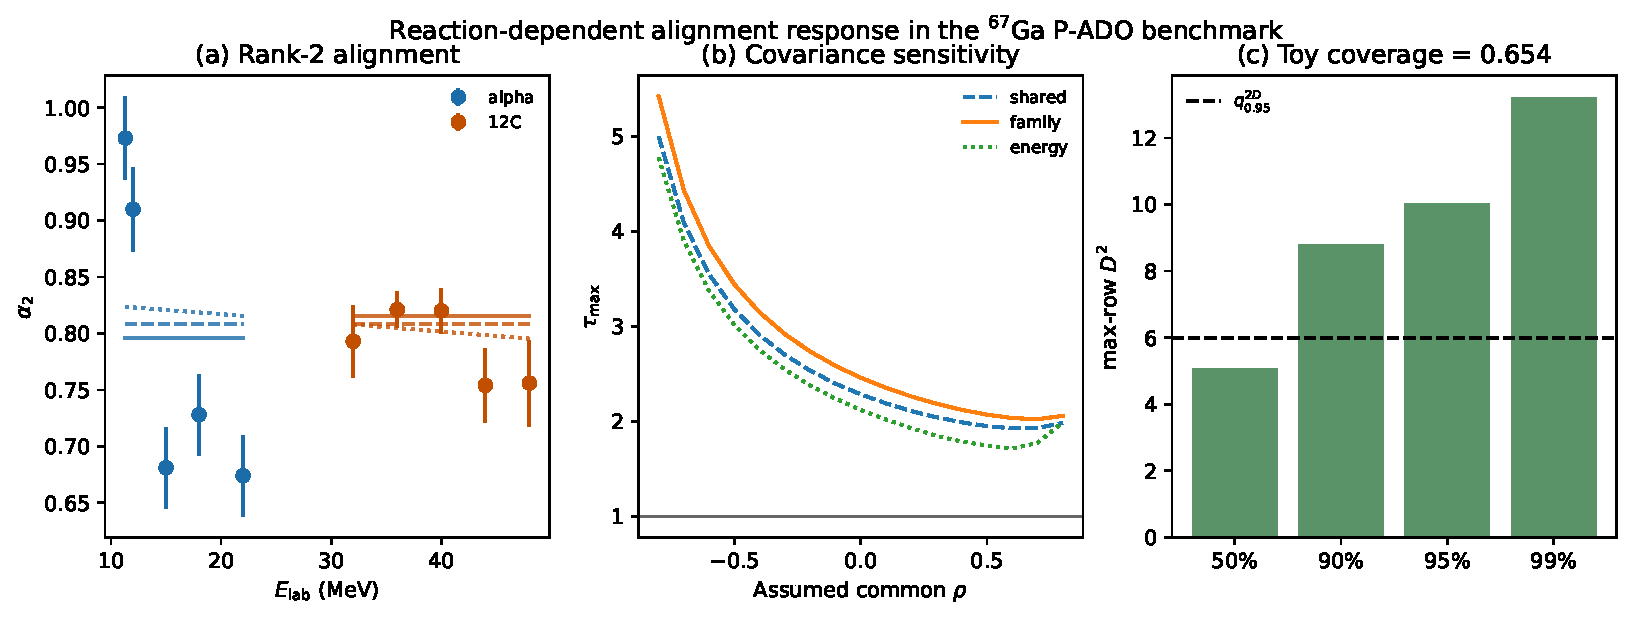
\includegraphics[width=\textwidth]{figures/alignment_response_profile.pdf}
\caption{(a) Published \(\alpha_2\) values and quoted marginal errors for the two projectile families, with the three response models and the separate mixture control. (b) Maximum-row discrepancy scale \(\tau_{\max}\) as a function of the assumed common row correlation \(\rho\). (c) Quantiles of the maximum-row \(D^2\) statistic in shared-null pseudo-experiments.}
\label{fig:profile}
\end{figure*}

\subsection{Coverage of the maximum-row threshold}

We generated 1000 pseudo-experiments from the shared model with \(r=0.28\), \(\rho=0\), and the row-specific quoted marginal errors. In each pseudo-experiment, \(r\) was refitted and the maximum row-wise \(D^2\) was calculated. The single-row two-dimensional threshold \(q_{0.95}^{(2)}=5.9915\) was satisfied in \(65.4\%\) of pseudo-experiments (Monte Carlo standard error \(0.015\)). The empirical 95th percentile of the maximum statistic was \(10.01\), rather than \(5.99\).

This result does not by itself calibrate the profiled statistic used for the observed
table. It changes the interpretation of a nominal threshold: applying a single-row
95\% contour to the maximum over ten rows is not a 95\% family-wise test. A
publication-level rejection or acceptance statement requires a predeclared
family-wise statistic, an event-level likelihood, or a coverage-calibrated test.

\subsection{Profile-preserving calibration}

To calibrate the statistic used for the observed covariance sensitivity, we repeated
the full \(\rho\)-profile and maximum-row operation in each pseudo-experiment. With
1000 pseudo-experiments for each true \(\rho\in\{-0.6,0,0.6\}\), the empirical
95th quantiles of the profiled statistic were \(8.79\), \(8.56\), and \(8.47\),
respectively. The observed profiled value is \(22.18\). This comparison is still
conditional on the independent-row Gaussian contract and the finite profile grid;
it is not an experimental p-value or a supremum calibration over all covariance
structures.

\subsection{Coverage sensitivity to the true alignment and covariance}

We extended the fixed-\(\rho\) sensitivity study over five true values of \(r\) from
0.10 to 0.60 and seven true row correlations from \(-0.8\) to \(0.8\), with 1000
pseudo-experiments per cell. When the fitted covariance matched the generating
covariance, the empirical coverage of the single-row threshold was approximately
0.62--0.68.
When the data were generated with a nonzero correlation but the fit forced
\(\rho=0\), the coverage fell as low as 0.47 at the edge of the scanned
negative-correlation range and was also below 0.53 in several other cells. The
nominal threshold is therefore
not stable under either the ten-row maximum operation or modest covariance
misspecification.

For comparison, the smallest observed shared-model \(D_{\max}^2\) across the
profile grid \(-0.8\leq\rho\leq0.8\) with spacing \(\Delta\rho=0.02\) is
\(22.18\), at \(\rho=0.64\). The fixed-\(\rho\) toy 95th percentiles range from
about \(9.60\) to \(10.59\) across the expanded sensitivity grid. This is a
finite-grid sensitivity result; the profile-preserving calibration above is the
relevant calibration for the observed profiled statistic.

\begin{figure*}[t]
\centering
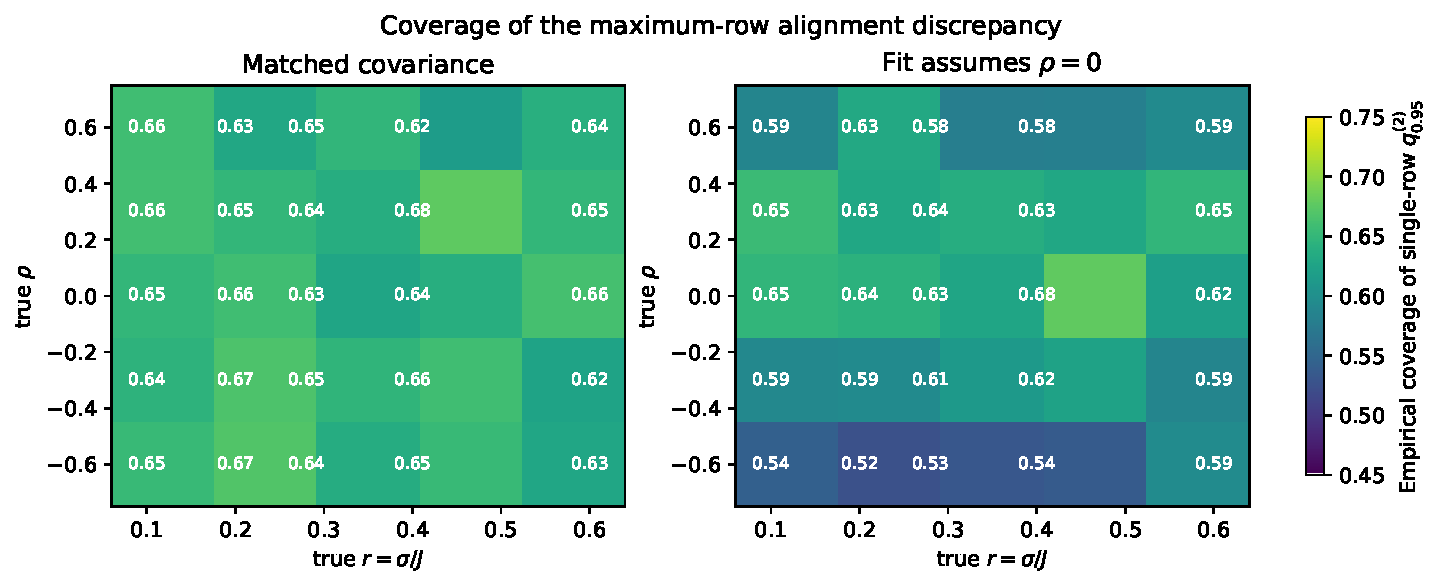
\includegraphics[width=\textwidth]{figures/coverage_grid.pdf}
\caption{Coverage of the single-row two-dimensional threshold for the maximum
over ten rows in a \(5\times7\) fixed-\(\rho\) toy grid. The left panel uses the generating
correlation in the fit; the right panel forces \(\rho=0\) while varying the
generating correlation. Values are empirical fractions from 1000 toys per cell.}
\label{fig:coverage-grid}
\end{figure*}

\section{Implications for A\(\approx130\) collective-mode spectroscopy}

The benchmark has a direct methodological consequence for A\(\approx130\) studies. ADO, DCO, polarization, and mixing-ratio analyses often combine information from different reaction conditions or inherit an alignment width from a reference transition. Zobel's experiment provides the physical reason to question that transfer: direct feeding and cascade feeding can change with projectile and beam energy \cite{Zobel1983}. The present calculation adds a quantitative layer by showing that the shared-response assumption can fail at the level of a multi-row observable vector, while a naive single-row threshold can have poor family-wise coverage.

The result does not select wobbling, tilted precession, chirality, or signature-partner bands in any particular A\(\approx130\) nucleus. It supports a pre-analysis diagnostic: a mixing-ratio branch used in collective-mode interpretation should retain condition-specific alignment nuisance, the \(\alpha_2\)--\(\alpha_4\) covariance, and a response or feeding control. Independent polarization or conversion-electron information remains necessary when the angular-distribution map has two real mixing-ratio roots \cite{Hamilton1975,Matta2015,Lv2022}.

\section{Limitations and next tests}

The missing row covariance is the dominant limitation. The table contains fitted coefficients, not raw spectra, so the present analysis cannot recover the covariance from first principles. The Gaussian population is also only one response model; a direct-plus-cascade mixture could explain part of the row-to-row variation, but the global convex mixture used here has no condition-specific feeding weights and does not validate a feeding mechanism. The energy-dependent and family models are descriptive alternatives, and the energy trend is confounded with projectile family in this fixture.

The next decisive test is a blind, event-level analysis with at least one pure-\(E2\) calibration line and several mixed transitions from the same acquisition. It should use the raw angular counts, on/off or sideband background terms, detector response, and a holdout transition. Pseudo-experiment coverage must be checked before a likelihood-ratio threshold is interpreted as a mode-selection significance. The present grid is a calibration sensitivity study, not a substitute for that event-level test.

\section{Conclusions}

The public \(^{67}\mathrm{Ga}\) P-ADO table is conditionally incompatible with a single shared alignment response under the stated table-level discrepancy contract. However, the data do not identify whether a family-specific or energy-dependent response is the correct replacement, and the nominal two-dimensional single-row threshold is not calibrated for the maximum over ten rows. The single transferable result is therefore a response and coverage requirement for mixing-ratio analyses that are later used to identify A\(\approx130\) collective modes.

\section*{Data availability}

The normalized ten-row benchmark table and all derived analysis outputs are included in
this local manuscript package. A public release should deposit the normalized CSV,
scripts, JSON outputs and a version identifier in a repository with a persistent
archive record. The source paper and its exact locator are recorded in the local
evidence record `knowledge/sources/zobel-1983-energy-projectile-alignment.md`; the
publisher PDF and raw event counts are not redistributed here. The source does not
provide row-internal or cross-row covariance, and no unavailable raw data are
claimed to have been reconstructed.

\section*{Code availability}

The profile, fixed-\(\rho\) coverage, profile-preserving calibration and coverage-grid
scripts are included under `analysis/` in this manuscript package. They use Python,
NumPy and SciPy; the fixed seeds, covariance contract and BIC row-unit convention
are recorded in the JSON results and README. The outputs are table-level analyses
and are not an event-level detector-response reanalysis.

\bibliography{references}

\end{document}
